\documentclass[tikz,border=2pt]{standalone}
\usepackage{lmodern}
\usepackage[T1]{fontenc}
\usepackage{amsmath,amssymb}
\usetikzlibrary{arrows.meta,calc,decorations.markings}

\definecolor{brownpop}{HTML}{D55E00}
\definecolor{tealpop}{HTML}{0072B2}
\definecolor{ink}{HTML}{222222}
\definecolor{muted}{HTML}{555555}
\definecolor{patch}{HTML}{E69F00}
\definecolor{boxfill}{HTML}{F4F7FA}
\definecolor{boxedge}{HTML}{C5CDD4}

\begin{document}
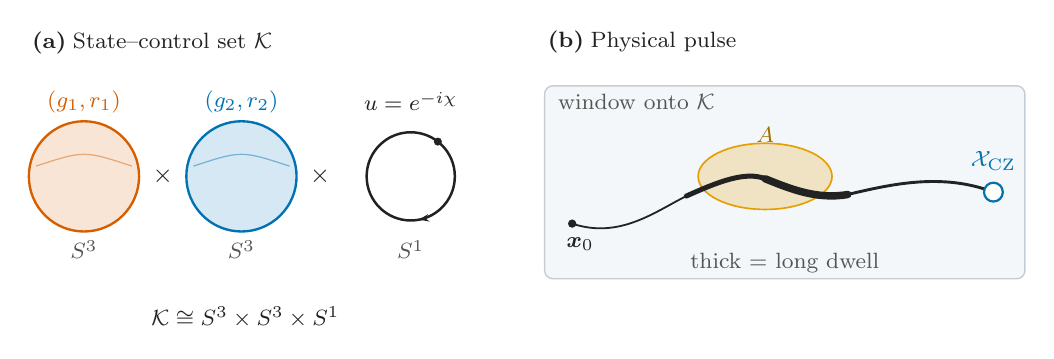
\begin{tikzpicture}[
  x=1cm, y=1cm,
  font=\fontsize{8}{9.6}\selectfont,
  >=Stealth,
  every node/.append style={inner sep=1pt},
]

% =================================================================
% (a)  content only; title is placed above the bounding box
% =================================================================
\begin{scope}[local bounding box=A]
  \fill[brownpop,opacity=0.16] (1.05,2.15) circle (0.70);
  \draw[brownpop, line width=0.85pt] (1.05,2.15) circle (0.70);
  \draw[brownpop, opacity=0.45, line width=0.45pt]
    (0.44,2.28) .. controls (1.05,2.48) .. (1.66,2.28);
  \node[text=brownpop] at (1.05,3.10) {$(g_1,r_1)$};
  \node[text=muted] at (1.05,1.22) {$S^3$};

  \node[font=\small, text=ink] at (2.05,2.15) {$\times$};

  \fill[tealpop,opacity=0.16] (3.05,2.15) circle (0.70);
  \draw[tealpop, line width=0.85pt] (3.05,2.15) circle (0.70);
  \draw[tealpop, opacity=0.45, line width=0.45pt]
    (2.44,2.28) .. controls (3.05,2.48) .. (3.66,2.28);
  \node[text=tealpop] at (3.05,3.10) {$(g_2,r_2)$};
  \node[text=muted] at (3.05,1.22) {$S^3$};

  \node[font=\small, text=ink] at (4.05,2.15) {$\times$};

  % Closed unit circle |u|=1; arrow on the ring (χ increases clockwise).
  \draw[ink, line width=0.90pt,
    decoration={markings,
      mark=at position 0.22 with {\arrow{Stealth[length=3.6pt]}}},
    postaction=decorate]
    ([shift={(5.20,2.15)}] 0:0.56) arc[start angle=0, end angle=-360, radius=0.56];
  \fill[ink] ([shift={(5.20,2.15)}] 52:0.56) circle (1.45pt);
  \node[text=ink] at (5.20,3.10) {$u=e^{-i\chi}$};
  \node[text=muted] at (5.20,1.22) {$S^1$};

  \node[text=ink] at (3.10,0.36)
    {$\mathcal{K}\cong S^3\times S^3\times S^1$};
\end{scope}

\node[anchor=south west, font=\fontsize{8}{9.6}\selectfont, text=ink]
  at ($(A.north west)+(0,0.38)$)
  {\textbf{(a)}\;State--control set $\mathcal{K}$};

% =================================================================
% (b)
% =================================================================
\begin{scope}[shift={(6.85,0)}, local bounding box=B]
  \draw[boxedge, fill=boxfill, rounded corners=3pt, line width=0.5pt]
    (0.05,0.85) rectangle (6.15,3.30);

  \node[anchor=west, text=muted] at (0.18,3.10) {window onto $\mathcal{K}$};

  \fill[patch, opacity=0.22] (2.85,2.15) ellipse (0.85 and 0.42);
  \draw[patch, line width=0.6pt] (2.85,2.15) ellipse (0.85 and 0.42);
  \node[text=patch!70!black] at (2.85,2.68) {$A$};

  \draw[ink, line width=0.65pt, line cap=round]
    (0.40,1.55) .. controls (1.00,1.35) and (1.45,1.70) .. (1.85,1.90);
  \draw[ink, line width=1.8pt, line cap=round]
    (1.85,1.90) .. controls (2.25,2.08) and (2.60,2.22) .. (2.85,2.12);
  \draw[ink, line width=2.7pt, line cap=round]
    (2.85,2.12) .. controls (3.15,2.00) and (3.50,1.85) .. (3.90,1.92);
  \draw[ink, line width=1.05pt, line cap=round]
    (3.90,1.92) .. controls (4.45,2.05) and (5.10,2.20) .. (5.75,1.95);

  \fill[ink] (0.40,1.55) circle (1.5pt);
  \node[anchor=north, text=ink] at (0.50,1.42) {$\boldsymbol{x}_0$};

  \draw[tealpop, line width=0.8pt, fill=white] (5.75,1.95) circle (3.4pt);
  \node[anchor=south, text=tealpop] at (5.75,2.18) {$\mathcal{X}_{\mathrm{CZ}}$};

  \node[text=muted] at (3.10,1.05) {thick $=$ long dwell};
\end{scope}

\node[anchor=south west, font=\fontsize{8}{9.6}\selectfont, text=ink]
  at ($(B.north west)+(0,0.38)$)
  {\textbf{(b)}\;Physical pulse};

\end{tikzpicture}
\end{document}
